\section{Einleitung} % (fold)
\label{sec:einleitung}

Laser sind in der heutigen Welt aus vielen Bereichen des modernen Lebens nicht mehr wegzudenken.
Es ist daher sinnvoll ein Verständnis für die Funktionsweise zu entwickeln.
Dieser Versuch soll genau dies gewährleisten.

\section{Theorie} % (fold)
\label{sec:theorie}

\subsection{Funktionsweise} % (fold)
\label{sub:was_ist_ein_laser_}

Ein Laser emittiert mochochromatisches Licht hoher Intensität und Kohärenz.
Dies wird mithilfe einer Pumpquelle, einem aktiven Lasermedium und einem Resonator erzeugt, wobei die Wellenlänge vom Lasermedium abhängt.

Das Lasermedium hat im einfachsten Fall zwei mögliche Energiezustände, deren Besetzung durch die Besetzungszahlen $n_1$ und $n_2$ beschrieben werden.
Tritt ein Photon in das Medium ein und besitzt eine höhere Energie als der Energieabstand zwischen den beiden Zuständen groß ist, kann es die Atome aus dem Grundzustand in den angeregten Zustand heben.
Ein angeregtes Atom kann spontan in den Grundzustand zurückkehren und dabei ein Photon emittieren, welches die Energiedifferenz der Zustände als Energie erhält.
Zudem kann aber auch ein weiteres einfallendes Photon zu einer stimulierten Emission führen, wobei das nun emittierte Photon dieselbe Energie, Phase und Ausbreitungsrichtung wie das einfallende besitzt.
Ein Schema ist in Abbildung \ref{Emission} dargestellt.

\begin{figure}[h!]
	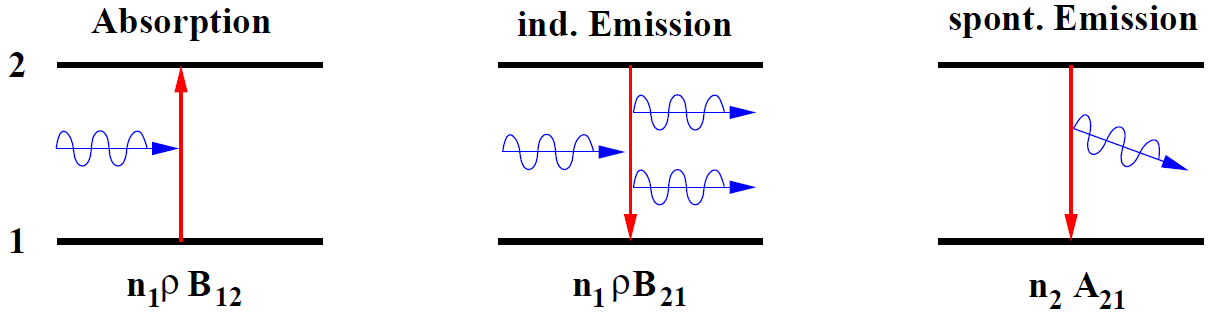
\includegraphics[width = 12cm]{pic/Emission.png}
	\label{Emission}
\end{figure}

Die Übergänge sind dabei von den Einsteinkoeffizienten $A_{21}$, $B_{21}$, $B_{12}$ und der Strahlungsdichte $\rho$ abhängig.
Dabei beschreibt die Ratengleichung den zeitlichen Verlauf der Besetzungsdichten $n_1$ und $n_2$ durch
\begin{align*}
	\frac{\mathrm{d}n_1}{\mathrm{d}t} = -n_1 B_{12} \rho + N_2 B_{21} \rho + n_2 A_{21}\,,\\
	\frac{\mathrm{d}n_2}{\mathrm{d}t} = +N_1 B_{12} \rho - n_2 B_{21} \rho - n_2 A_{21}\,.
\end{align*}
Dabei ist $N_i$ die Anzahl der emittierten/absorbierten Photonen.

Damit der Laser Funktioniert muss gegeben sein:
\begin{itemize}
	\item Mehr Atome im angeregten Zustand als im Grundzustand (Besetzungsinversion)
	\item Mehr Verstärkung als Verluste.
\end{itemize}

Um 1) zu erreichen muss dem Lasermedium über die Pumpquelle kontinuierlich Energie zugeführt werden.
Beim Helium-Neon Laser werden die Helium Atome in Metastabile Zustände angeregt.
Diese regen über Stöße zweiter Art die Neon Atome an, welche über spontane Emission die ersten Photonen emittieren.

Damit die Verstärkung größer ist als die Verluste, werden die emittierten Photonen mithilfe eines Resonators viele male durch das Lasermedium gelenkt, wodurch die Verstärkung exponentiell mit der Länge des Laufweges im aktiven Lasermedium ansteigt.
Der Resonator besteht aus sich gegenüberliegenden Spiegeln.
Damit der Laser ausgekoppelt werden kann, ist einer davon zu einem geringen Teil durchlässig, während der andere optimalerweise nicht durchlässig sein sollte.
Der Stabilitätsparamter beschreibt dabei, ob die Verstärkung die Verluste ausgleichen kann oder nicht. 
Er ist durch 
\begin{equation*}
	g_1 g_2 = (1-L/r_1)(1-L/r_2)
\end{equation*}
gegeben.
Dabei ist $r_i$ der Krümmungsradius des Spiegels und $L$ die Länge des Resonators.

\subsection{Gaußverbreiterung}
\label{subsec:gaußverbreiterung}
Ein unwillkommener Effekt für Anwendung von Gaslasern in der Spektroskopie ist
die Gaußverbreiterung.
Neben der natürlichen Linienbreite wird das Frequenzspektrum des Laserlichtes
von dieser überlagert.
Auf Grund der statistisch verteilten, relativen Bewegungsrichtung der
Gasmoleküle im HeNe-Plasma, erscheinen die Schwingungsfrequenzen $f$ dieser
Moleküle verschoben.
Die Geschwindigkeitsverteilung ist dabei durch die Maxwell-Boltzmann-Verteilung
gegeben. Die Breite dieser Verteilung beträgt
\begin{equation}
\label{eq:sigma_maxwell_boltzmann}
    \sigma_f = \frac{f_0}{\mathrm{c}}\sqrt{\frac{\mathrm{k}_\text{B}T}{m}}\,,
\end{equation}
wobei $f_0$ die Grundfrequenz bezeichnet und $m$ die Masse des Moleküls.
